\section{Reproduction of two macrobenchmarks}

We decided to attempt reproducing two macrobenchmarks with an IO-heavy workload on the Distributed ASCI Supercomputer 5 (DAS-5). DAS-5 is a six-cluster wide-area distributed system designed by the Advanced School for Computing and Imaging.

This section will go into more detail for the two experiments we chose to reproduce. Furthermore, we will review our reproduction steps, challenges encountered, and the results of the experiments.

\subsection{IO-heavy workload --- comparing running times}

We chose to reproduce the experiments where the authors compared the running time's cumulative distribution function (CDF) of a FIFO scheduler, a scheduler utilising na\"{i}ve fair scheduling and a scheduler using both fair and delay scheduling. The results the authors achieved in their paper can be seen in Figure \ref{fig:original_5}. It is apparent that the scheduler using FIFO fares significantly worse in the lower 8 bins than both the scheduler utilising na\"{i}ve fair scheduling and the scheduler using both fair and delay scheduling. However, the very long running tasks (in bin 9) are hindered by the presence of fairness.

We decided to focus on this experiment in particular since it did not show there to be a significant difference between the na\"{i}ve fair scheduler and the one using delay scheduling. We wanted to double-check their results to see if the difference is this slim and possibly due to different circumstances since Zaharia et al. presumably did not repeat it multiple times.

\begin{figure}
  \centering
  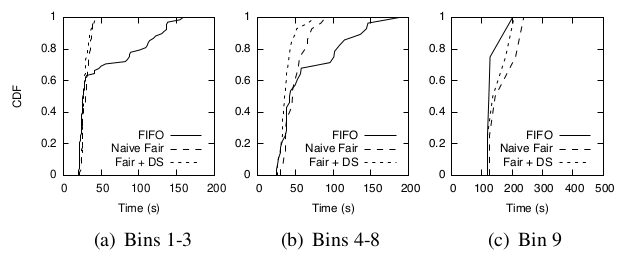
\includegraphics[width=\linewidth]{figures/figure_5.png}
  \caption{CDFs of running times of jobs in various bin ranges in the IO-heavy workload. Fair sharing greatly improves performance for small jobs, at the cost of slowing the largest jobs. Delay scheduling further improves performance, especially for medium-sized jobs. From the original paper \cite{ds}.}
  \label{fig:original_5}
\end{figure}


\subsection{Obstacles}

One of the first challenges was to figure out the exact experiments the original authors ran. They refer to the benchmarks described by Zheng Shao \cite{shao_2009}. However, the purpose of this suite is to compare three different data processing systems, including Hadoop and Hive. Since Hive is built on top of Hadoop and many of the authors are from Facebook solving a problem affecting their company\footnote{The company responsible for Hive and also utilising it to a great extent.}, it is safe to assume that they used the Hive benchmarks for evaluation purposes.

Building these benchmarks as Java programs was also the cause of great frustration. This was probably due to the sparse documentation and the 12 years that have passed since the publication of the original code. However, after figuring out the exact library versions to use, environment variables to set, and the Perl programming language, we have grown to like the benchmark program.

\subsection{Our setup}

We created a Python script for allocating a given number of nodes, and downloading and installing Hadoop and Hive on them. A master node is selected on which Derby is also installed and the Hadoop NameNode, YARN, history server, Hive, and Derby are configured. On all the nodes, HDFS \cite{borthakur2007hadoop} is also configured. The script continuously maintains an SSH connection with the master node, on the failure of this connection, or an interrupt, it cleans up all the nodes used: the processes are stopped and the data is destroyed.

Another script is responsible for running the Hive version of the \texttt{grep} benchmark from \cite{shao_2009} many times. The length of the datasets is each time determined by a distribution similar to the original experiment's input distribution. Nevertheless, we had far less resources at our disposal, hence, we took the liberty to scale down the sizes which can be seen in Table \ref{tab1}. Although we could have used more, we chose to only utilise 12 nodes for the experiments. Since we were not the only group working on this assignment, we refrained from hogging all the available nodes for extended periods of time.

\begin{table}
\centering
\caption{Distribution of job sizes}\label{tab1}
\begin{tabular}{|l|l|l|l|}
\hline
\textbf{Bin} & \textbf{Maps} & \textbf{Jobs} \\ \hline
0  & 1 & 19       \\ \hline
1  & 2 & 8       \\ \hline
2  & 10 & 7       \\ \hline
3  & 50 & 4       \\ \hline
4  & 100 & 3       \\ \hline
5  & 200 & 2       \\ \hline
6  & 400 & 2       \\ \hline
7  & 1200 & 2       \\ \hline
\end{tabular}
\end{table}

The aforementioned script saves the statistics of each map task into a separate output file. These are then converted to \texttt{JSON} documents that only contain the relevant information and can be subsequently plotted using the rest of our Python scripts. 

\subsection{Our results}

\begin{figure}
  \centering
  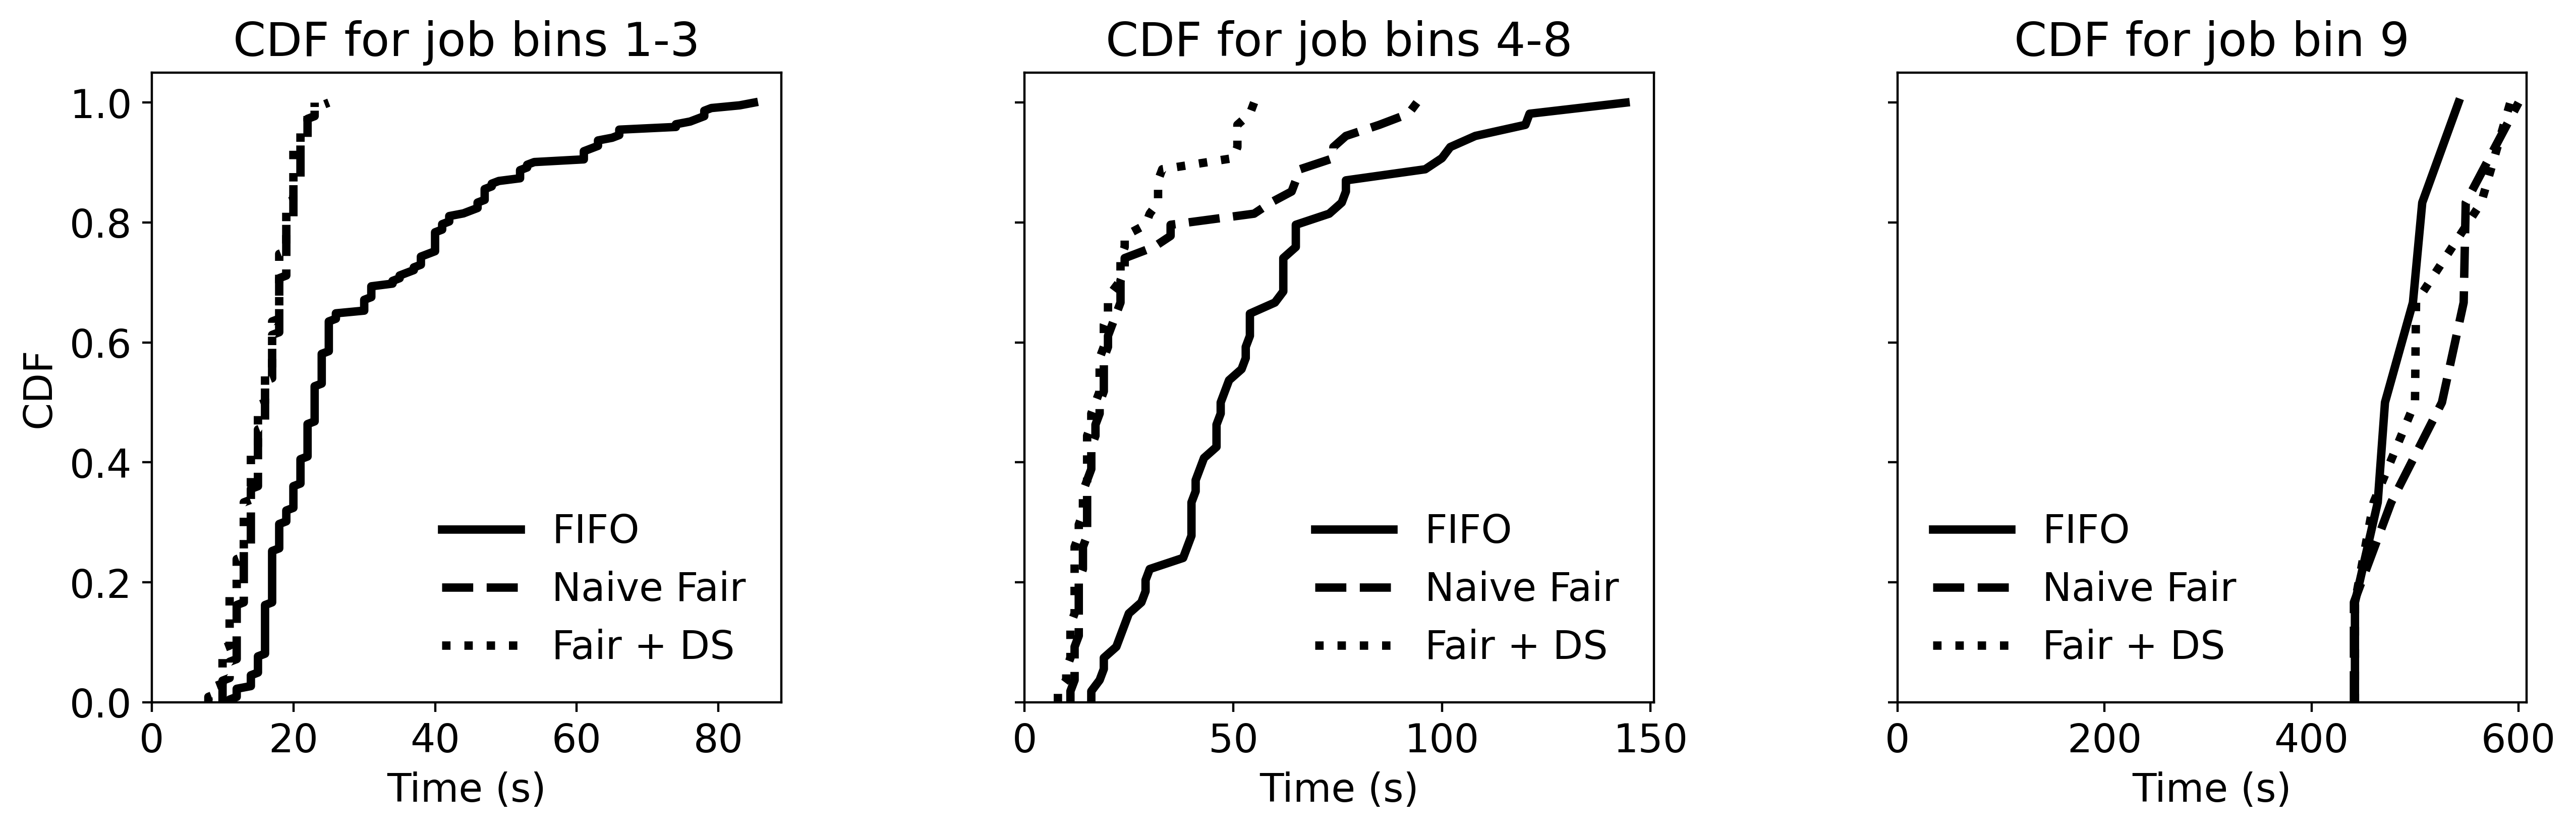
\includegraphics[width=\linewidth]{figures/running-times.png}
  \caption{Our results for the experiment shown in Figure \ref{fig:original_5}. The bin numbering is from the original experiment's distribution.}
  \label{fig:reproduced_5}
\end{figure}


In Figure \ref{fig:reproduced_5}, we can see a surprisingly close resemblance to Figure \ref{fig:original_5}. We conclude that we and Zaharia et al. \cite{ds} must have done very similar steps\footnote{With the caveat, that our cluster setup --- similarly to the originals --- is also not representative of real life networking conditions: each node is located in the same rack.}. There are some noticeable differences though. We ran the experiment three times and used all tasks running times for the CDF, making our charts look smoother. Secondly, when it comes to the medium sized jobs, delay scheduling outperformed its naive counterpart\footnote{We used the Hadoop Fair Scheduler with its thresholds set to zero to implement this.} more noticeably.

\subsection{IO-heavy workload --- comparing speedup}

Using the logs of the aforementioned run, we did some further analysis. We were curious about the speedup gained from opting for a different scheduler. The authors' original analysis can be seen in Figure \ref{fig:original_10} and \ref{fig:original_7}. The results of our experiment are shown in Figure  \ref{fig:delay_vs_naive} and \ref{fig:delay_vs_fifo}. The similarity between Figure \ref{fig:original_7} and \ref{fig:delay_vs_naive} is convincing: the values are between around 1 and 1.5, and both shapes have 2 peaks (at bin 5 and 8, and at bin 2 and 5).

\begin{figure}
  \centering
  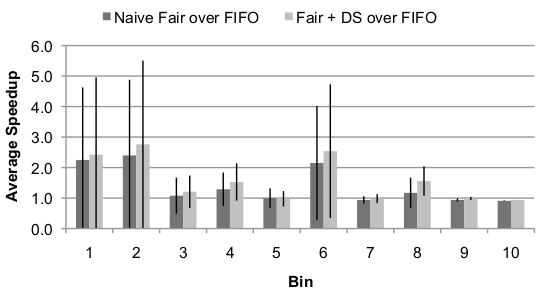
\includegraphics[width=\linewidth]{figures/figure_10.png}
  \caption{Average speedup of delay scheduling over na\"{i}ve fair sharing for jobs in each bin in the IO-heavy workload. The black lines show standard deviations. From the original paper \cite{ds}.}
  \label{fig:original_10}
\end{figure}

\begin{figure}
  \centering
  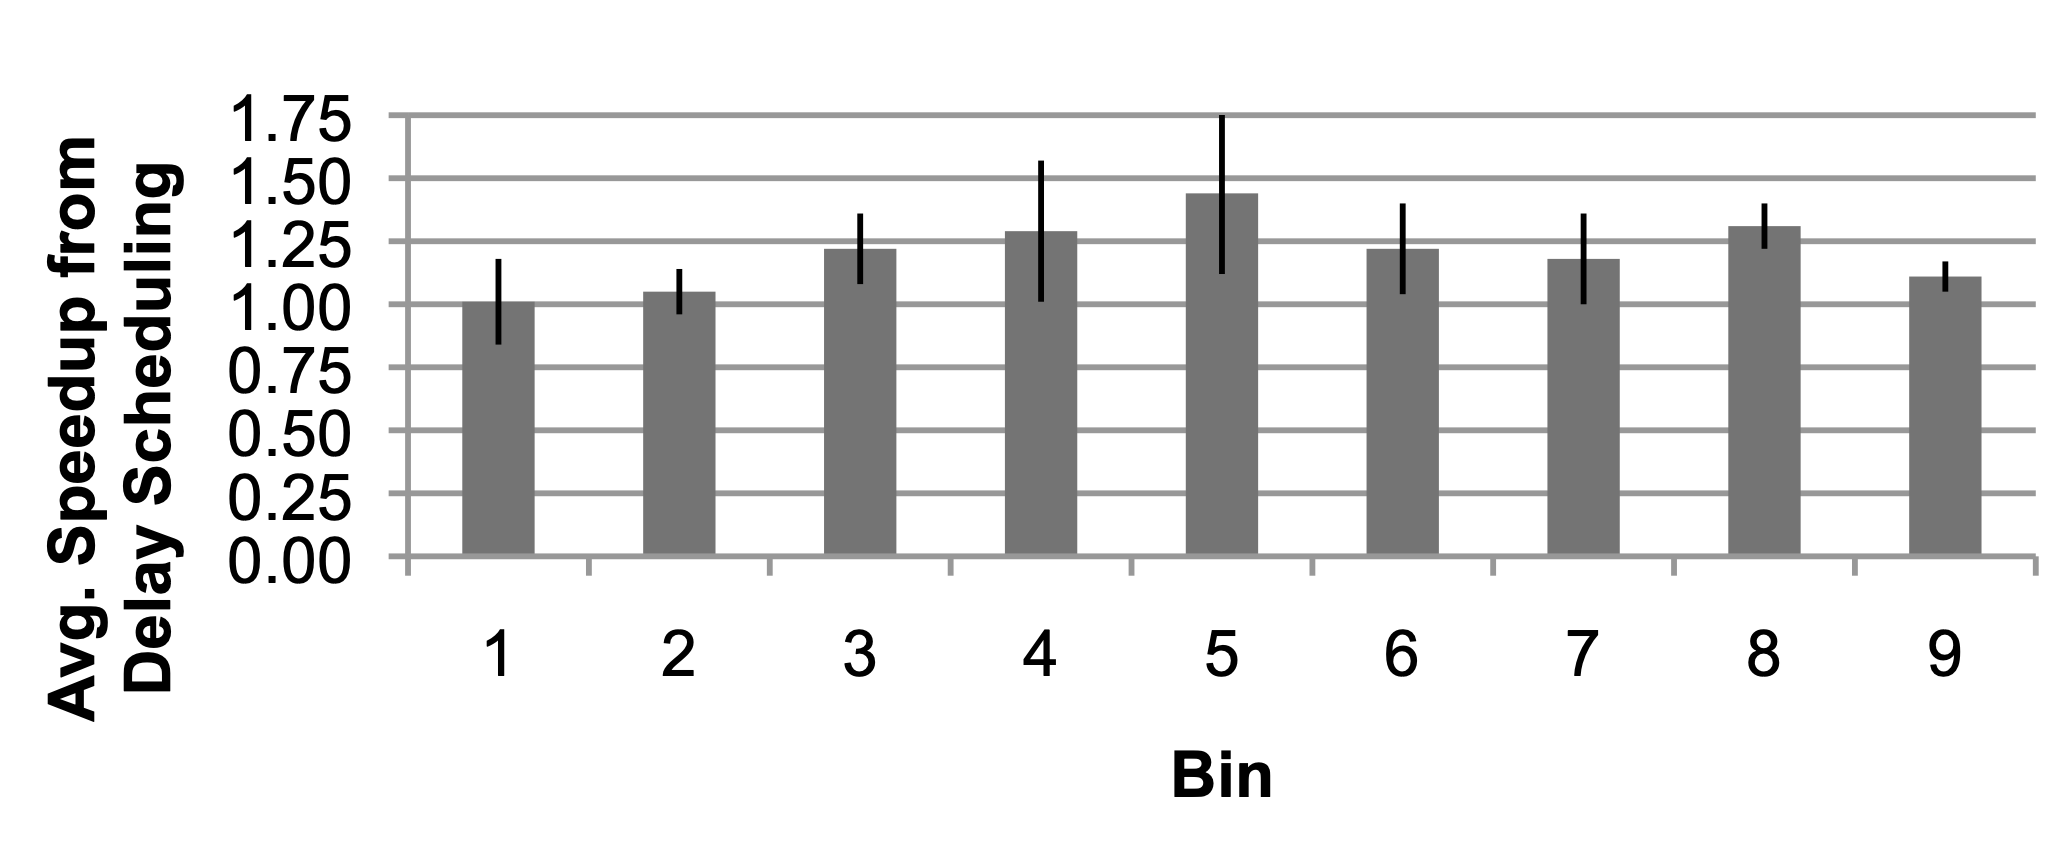
\includegraphics[width=\linewidth]{figures/figure_7.png}
  \caption{Average speedup of delay scheduling over naive fair sharing for jobs in each bin in the IO-heavy workload. The black lines show standard deviations. From the original paper \cite{ds}.}
  \label{fig:original_7}
\end{figure}


\begin{figure}
  \centering
  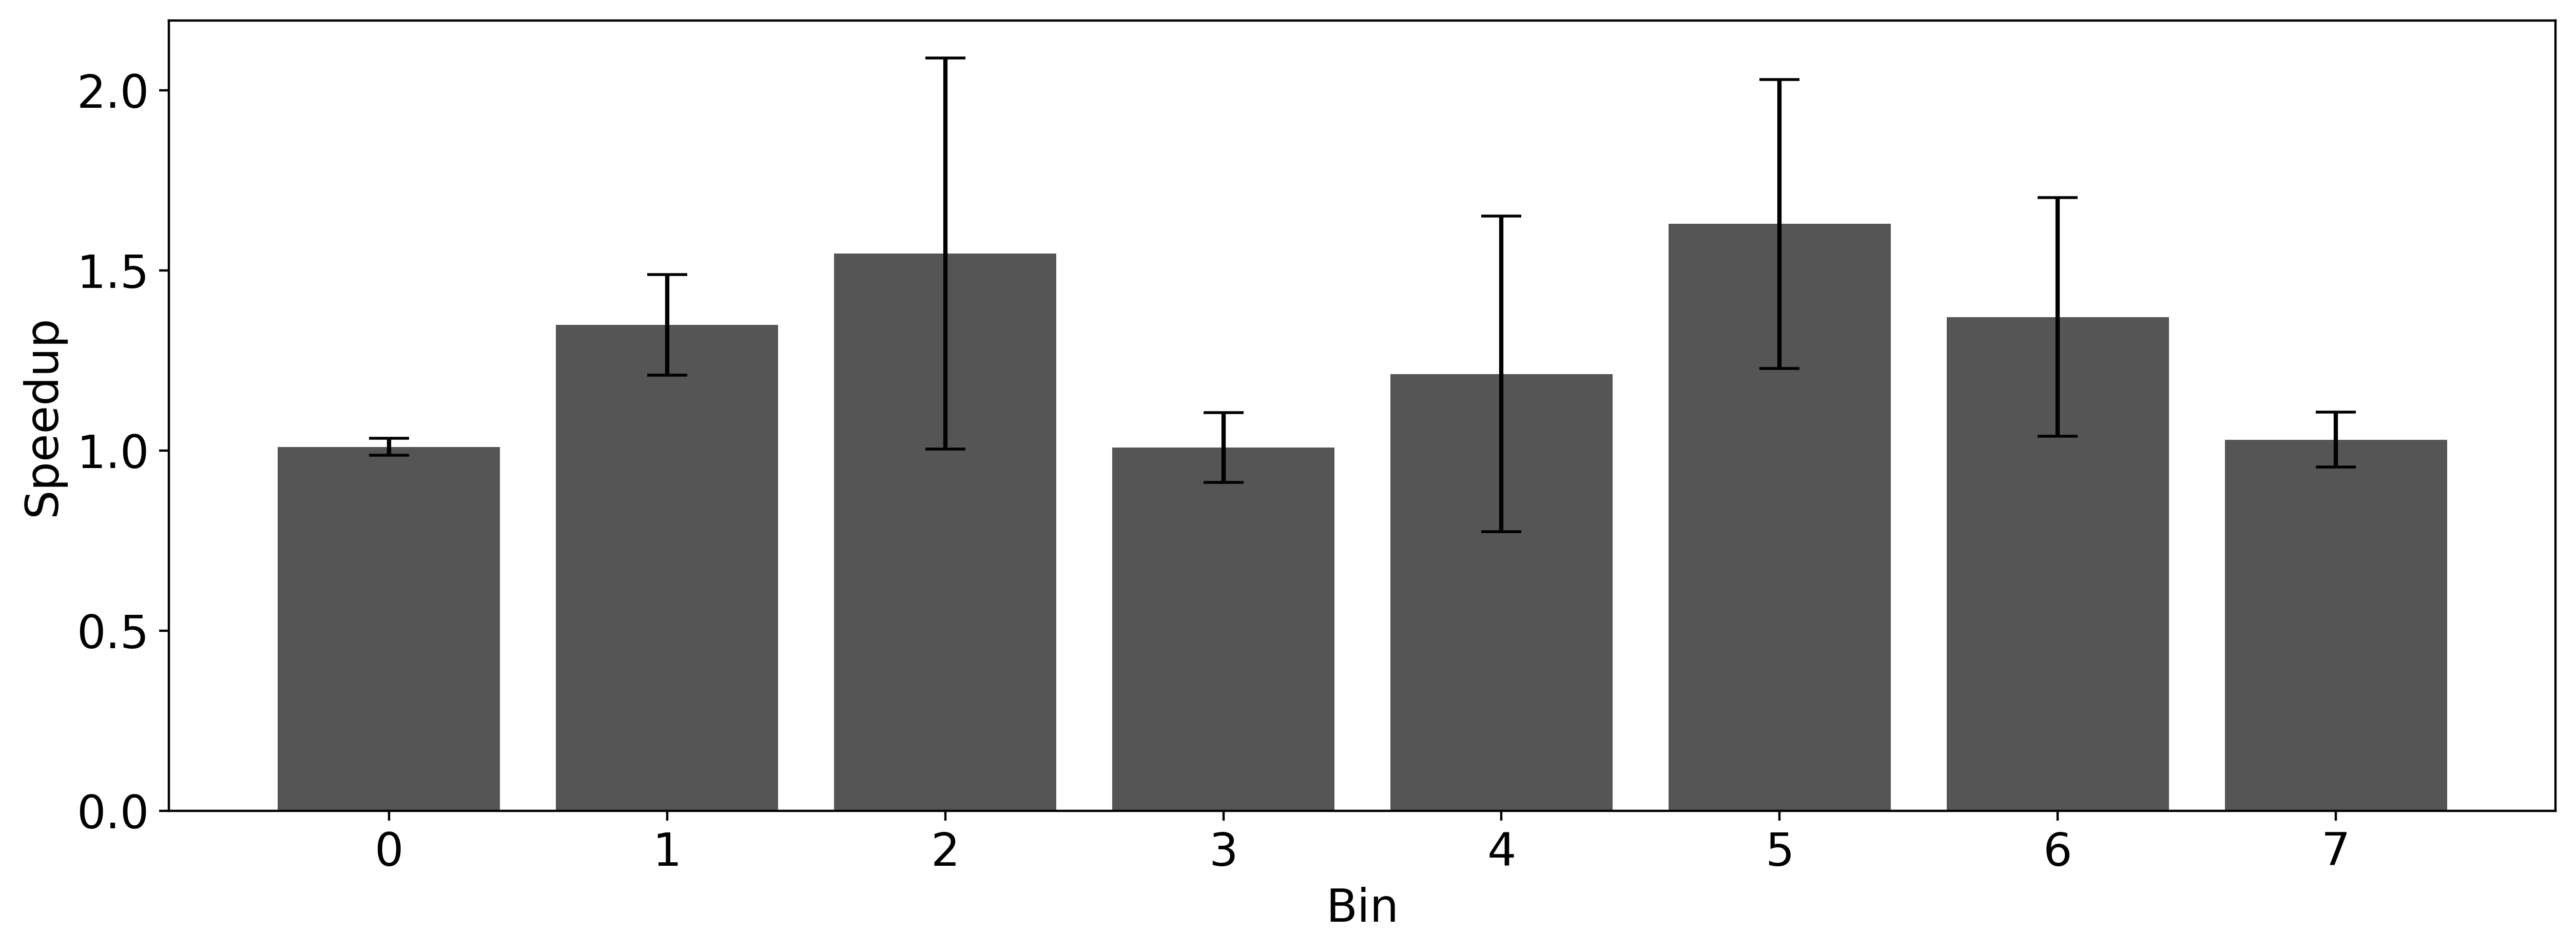
\includegraphics[width=\linewidth]{figures/delay-fair-speedup.png}
  \caption{Average speedup of delay scheduling over na\"{i}ve fair sharing for jobs in each bin in the IO-heavy workload.}
  \label{fig:delay_vs_naive}
\end{figure}

\begin{figure}
  \centering
  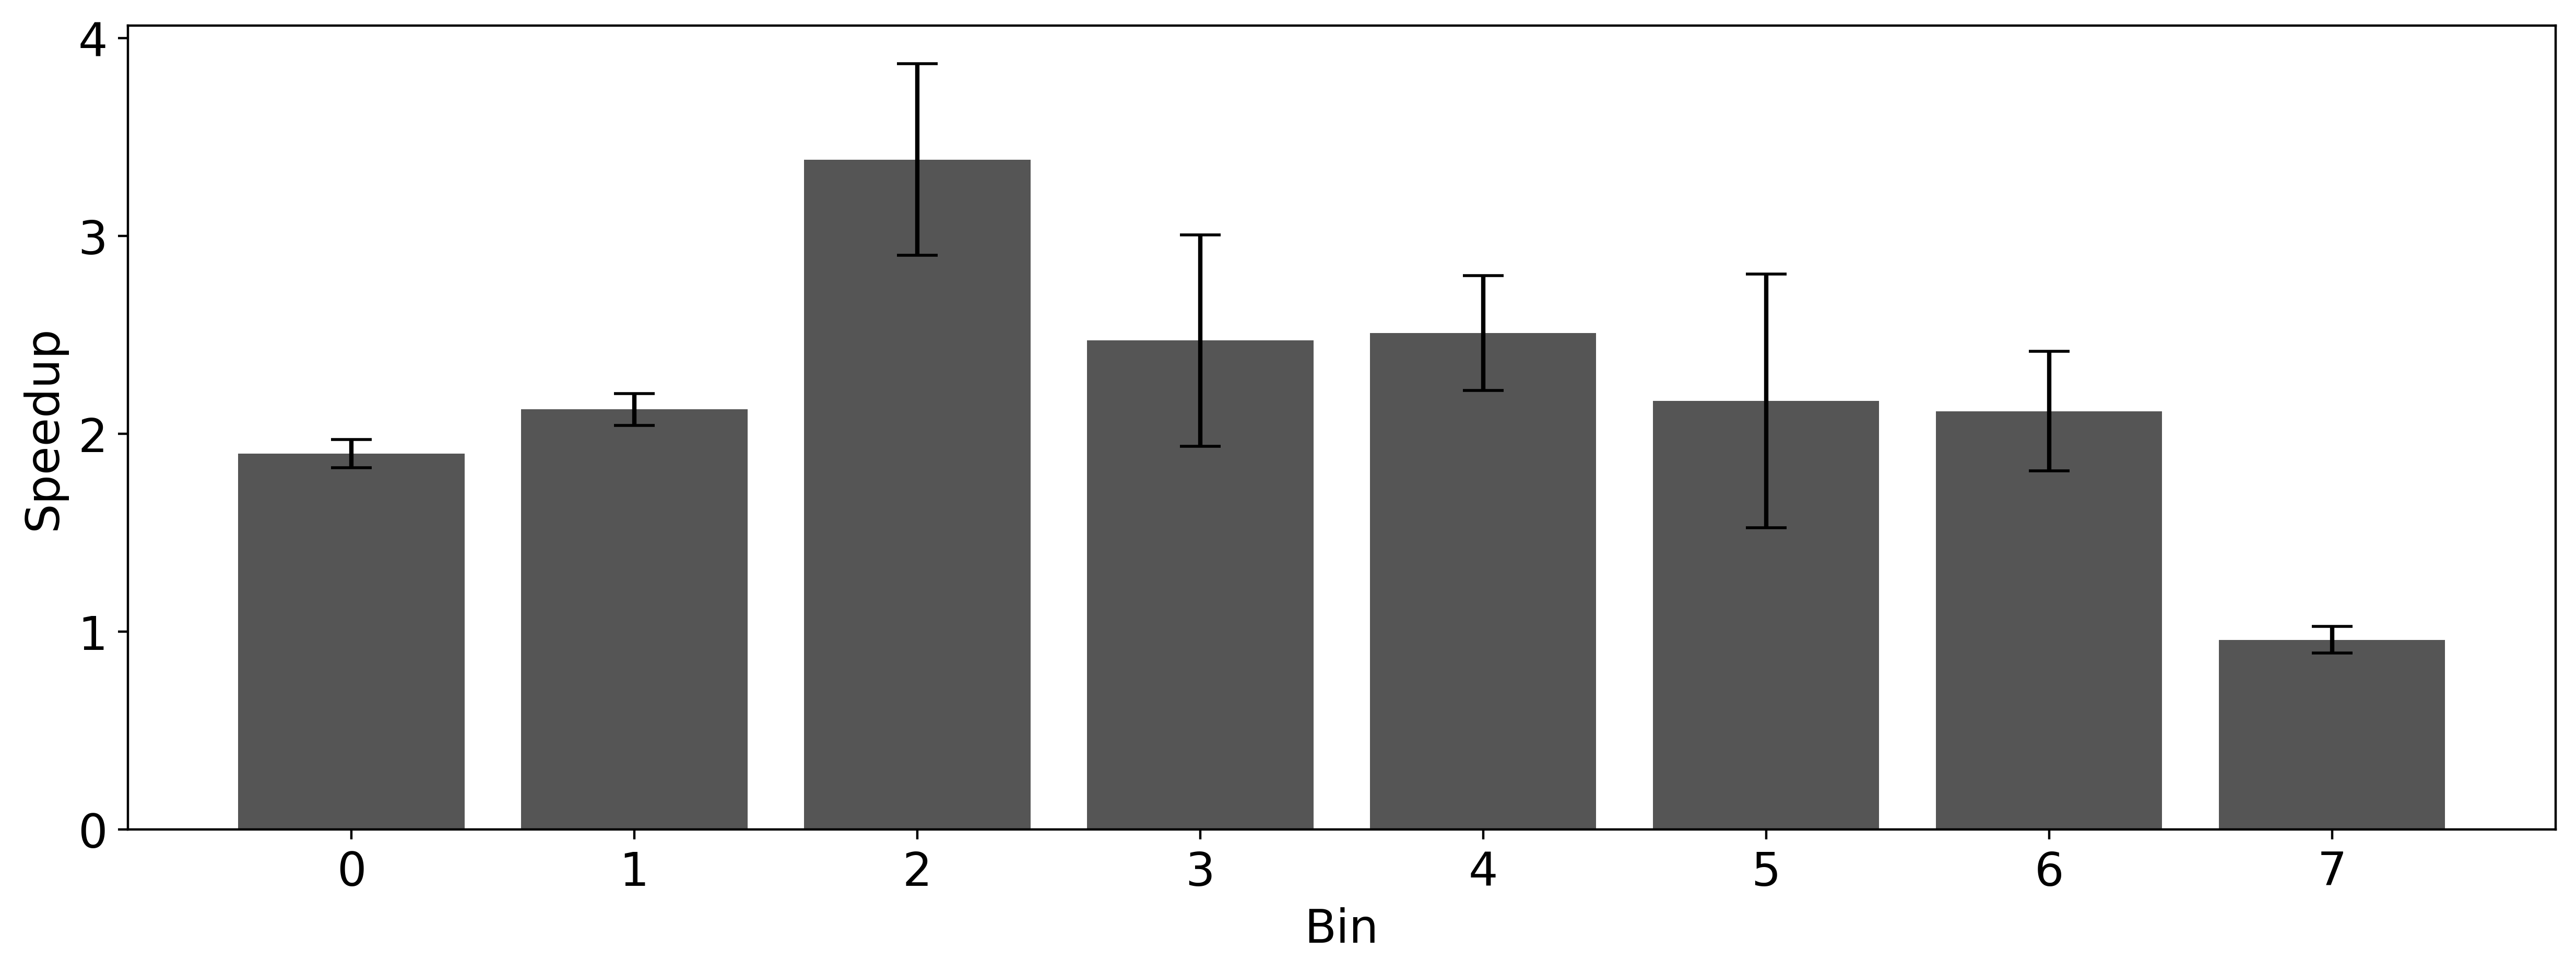
\includegraphics[width=\linewidth]{figures/delay-fifo-speedup.png}
  \caption{Average speedup of delay scheduling over FIFO scheduling for jobs in each bin in the IO-heavy workload.}
  \label{fig:delay_vs_fifo}
\end{figure}



However if we take a closer look at Figure \ref{fig:original_10}, the standard deviations are suspiciously large. In our evaluation, the outlier deviations are gone which might be the result of the multiple repetitions we had.

Overall, we gained more from abandoning the FIFO scheduler than Zaharia et al. We theorise, that this might be due to the smaller sized cluster where the scheduling opportunities are more rare as compared with their 100-node clusters. 

